\documentclass[aspectratio=169]{beamer}
\usepackage{standalone}

\usepackage{stmaryrd}
\usepackage{listings}
\usepackage{fontawesome}
\usepackage{bm}

\usepackage[hyperref=auto,style=alphabetic,backend=bibtex]{biblatex}
\addbibresource{kwarcpubs.bib}
\addbibresource{extpubs.bib}
\addbibresource{extcrossrefs.bib}
\addbibresource{bib.bib}
\addbibresource{examples.bib}
\usepackage{appendixnumberbeamer}
\usepackage{tikz}
\usepackage{tikz-qtree}
\usetikzlibrary{arrows.meta}
\usetikzlibrary{shapes}
\usetikzlibrary{mmt}
\usetikzlibrary{docicon}

\usetheme{Pittsburgh}
% \setbeamertemplate{footline}[frame number]
\setbeamertemplate{footline}{\hfill\insertframenumber\,/\,\inserttotalframenumber\quad\strut}
\setbeamertemplate{navigation symbols}{}
\usecolortheme{beaver}
\setbeamertemplate{frametitle}[default][left]
% \setbeamersize{text margin left=3em}

\usepackage{utils/colors}
\usepackage[forbeamer]{utils/basic}
\usepackage{utils/operators}
\usepackage{utils/mylstmisc}
\usepackage{utils/lstmmt}

\lstset{basicstyle=\ttfamily}
\lstset{commentstyle=\itshape\color{commentfont}}
\def\examplecite#1{{\textit{\color{black!60!blue}\small Example from \cite{#1}}}}

\title{Towards and Annotation Standard for STEM Documents \\\large Datasets, Benchmarks, and Spotters}


% rdf nodes
\tikzset{urinode/.style={draw, ellipse, minimum width=1.3cm, minimum height=0.6cm}}
\tikzset{typenode/.style={draw}}
\tikzset{bnode/.style={draw, ellipse, minimum width=1.0cm, minimum height=0.6cm}}
\tikzset{literal/.style={draw, rounded corners=0.1cm}}

% rdf edges
\tikzset{normaledge/.style={-Latex}}
\tikzset{typeedge/.style={arrows={-Latex[open]}}}

% custom nodes
\tikzset{body/.style={fill=green!50}}
\tikzset{target/.style={fill=blue!30}}
\tikzset{annotation/.style={fill=red!50}}


\author{\textbf{Jan Frederik Schaefer} \and Michael Kohlhase}
\institute{FAU Erlangen-N\"urnberg/KWARC}
\date{\textbf{Conference on Intelligent Computer Mathematics (CICM)}\\Cambridge, UK\\September 7, 2023}

\begin{document}
\frame\titlepage


\begin{frame}
    \frametitle{Natural Language Processing and Mathematical Language}
    \begin{itemize}
        \item Natural language processing has benefitted from a long tradition of annotation tasks and benchmarks
        \item STEM documents pose problems:
            formulae, tables, \textellipsis
            \com{not really unicode strings}
        \item Why care?\\
            $\leadsto$ Semantic services
    \end{itemize}
\end{frame}


\begin{frame}
    \frametitle{Motivation: semantic services}
    \faSearch\;\; $\bm{1.5\,\text{\bf eV}}$
    \\[1em]
        \quad\quad\faExternalLink\;\; $1.43 \pm 0.9\,\text{eV}$\\[1em]
        \quad\quad\faExternalLink\;\; $2.4 \cdot 10^{-19}\,J$

    \vspace{3em}
    \faSearch\;\; $\bm{\sum_{k=-\infty}^\infty \text{\bf exp}(-\pi k^2)}$
    \\[1em]
        \quad\quad\faExternalLink\;\; $\sum_{n=-\infty}^\infty e^{-\pi n^2} = \ldots$
\end{frame}


\begin{frame}
    \frametitle{Motivation: semantic services}
    \hfill \examplecite{krisciunas2022including}\par
    \centering
    \begin{tikzpicture}
    \node at (0, 0) {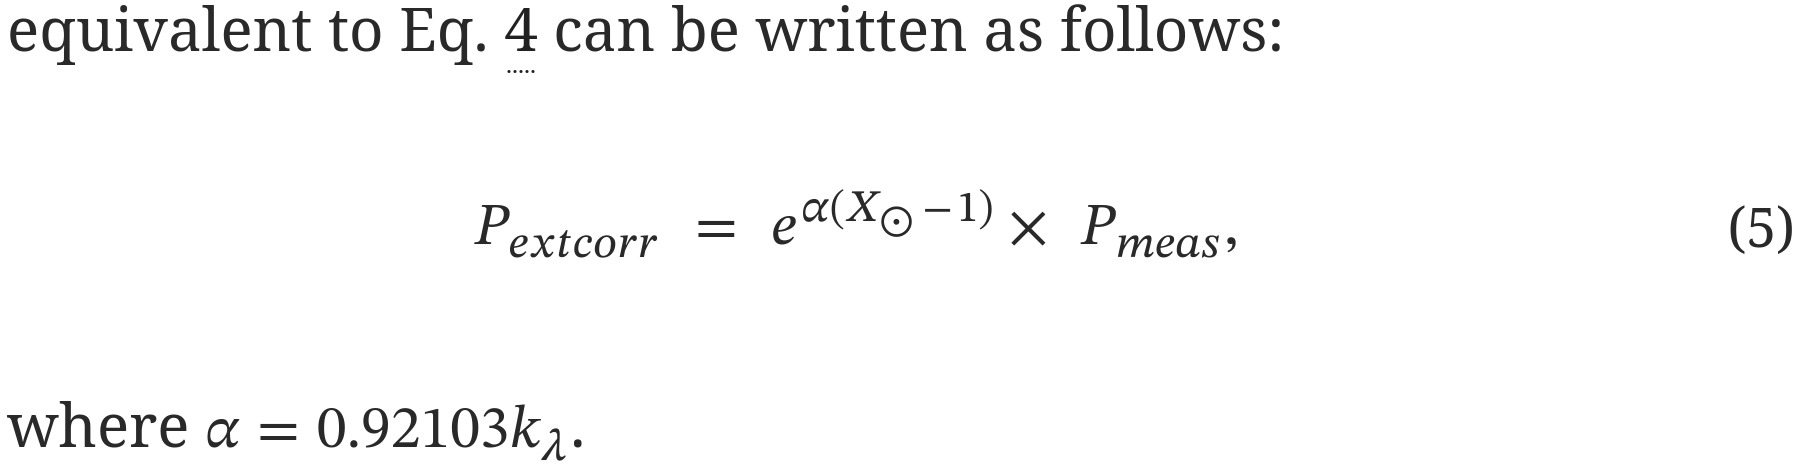
\includegraphics[width=0.8\textwidth]{extcorr_2107.02876.png}};
    \onslide<2>{\node at (1.6, -1.6) {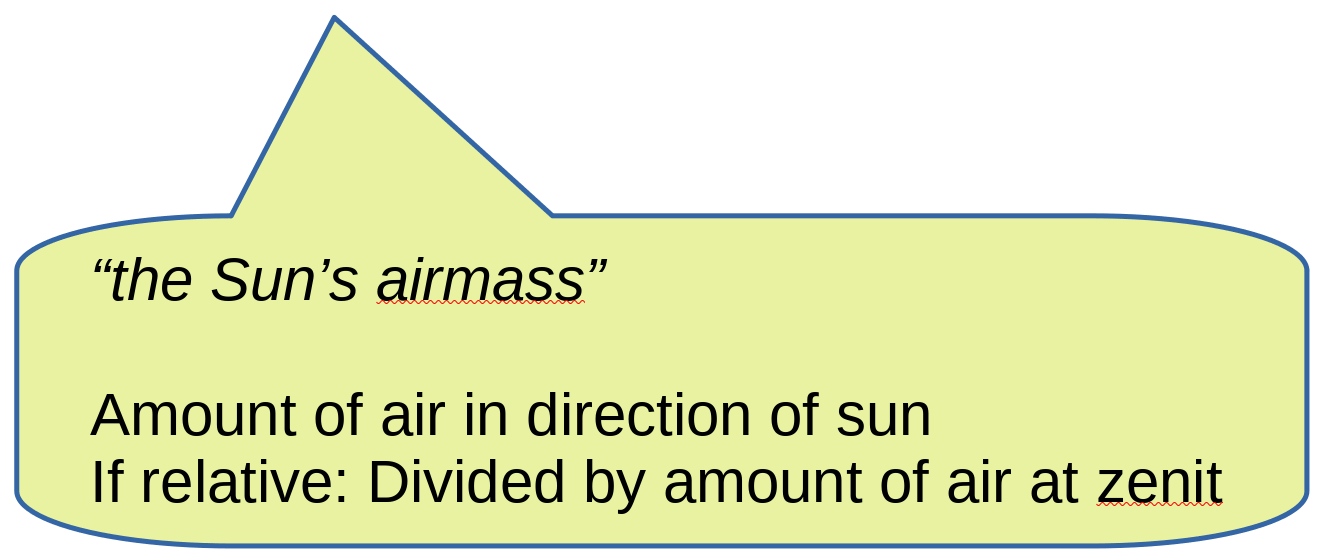
\includegraphics[width=0.5\textwidth]{bubble.png}};}
    \onslide<3>{\node at (1.5, -2.1) {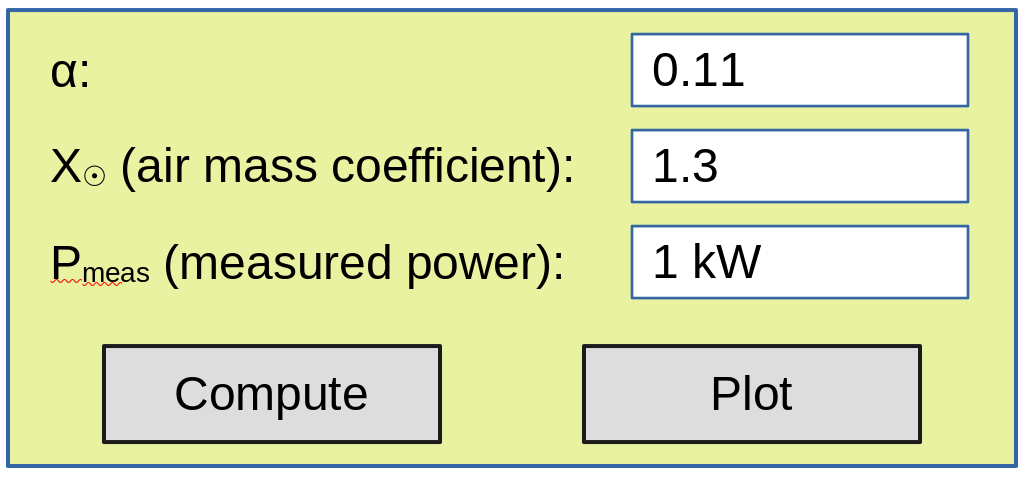
\includegraphics[width=0.5\textwidth]{compute.png}};}
    \end{tikzpicture}
%     \begin{itemize}
%         \item Computable formulae
%         \item Screen readers
%         \item Active documents
%         \item Formula search
%     \end{itemize}
\end{frame}


\begin{frame}
    \frametitle{Motivation: semantic services}
    \centering
    \Large
    For all those services\\
    {\bfseries we need semantic annotations!}\\\com{(full formalization not necessary)}
    \vspace{2em}\par
    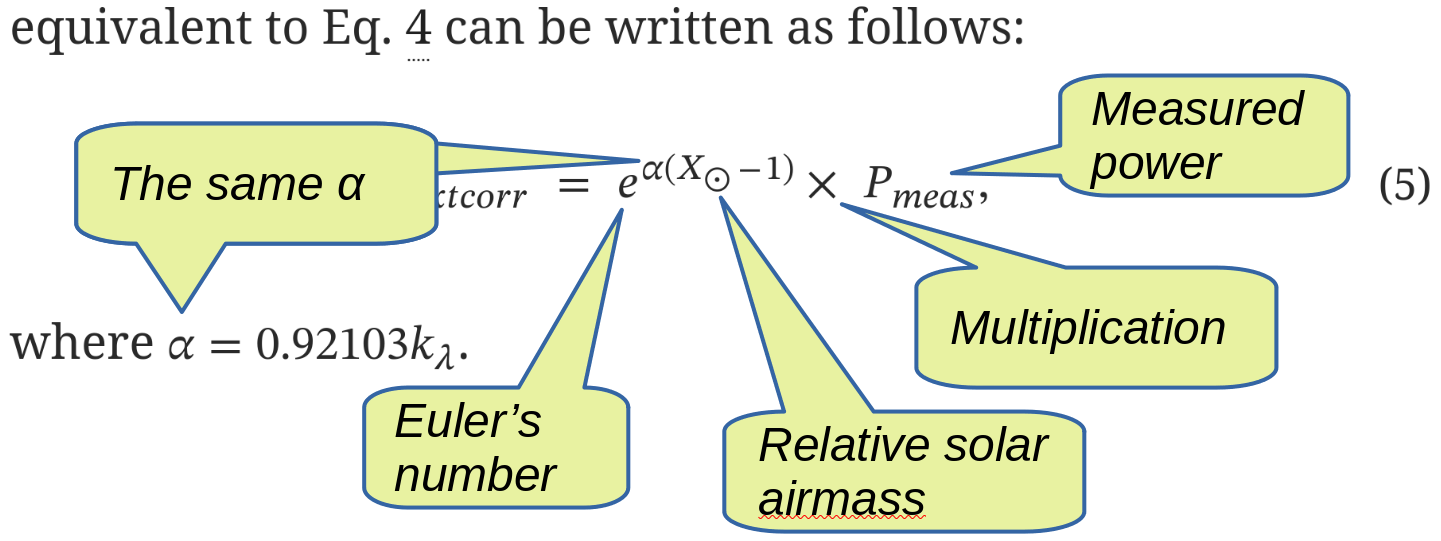
\includegraphics[width=0.5\textwidth]{annos.png}
    \vspace{2em}\par
    \pause
    Authors don't provide them $\leadsto$ We have to infer them
\end{frame}





\begin{frame}
    \frametitle{Accumulating semantic annotations with spotters}
    \centering
    \textbf{Spotter:} specialized tool for finding a particular type of annotation
    \vspace{2em}\par

    \begin{tikzpicture}[db/.style={cylinder, shape border rotate=90, draw, aspect=0.3,scale=4},spotter/.style={draw}]
        \node[db,thick] (db) at (0, 0) {};
        \node[spotter] (s1) at (-3, 1) {\begin{tabular}cParagraph\\classification\\spotter\end{tabular}};
        \node[spotter] (s2) at (3, 1.5) {\begin{tabular}cDeclaration\\spotter\end{tabular}};
        \node[spotter] (s3) at (3, -1.5) {\begin{tabular}cMath concept\\spotter\end{tabular}};
        \node[spotter] (s4) at (-3, -1.5) {\begin{tabular}cUnit\\spotter\end{tabular}};
        \draw[->] (s1) -- (db);
        \draw[->] (s2) -- (db);
        \draw[->] (s3) -- (db);
        \draw[->] (s4) -- (db);
        \node (doc) at (0, -4.5) {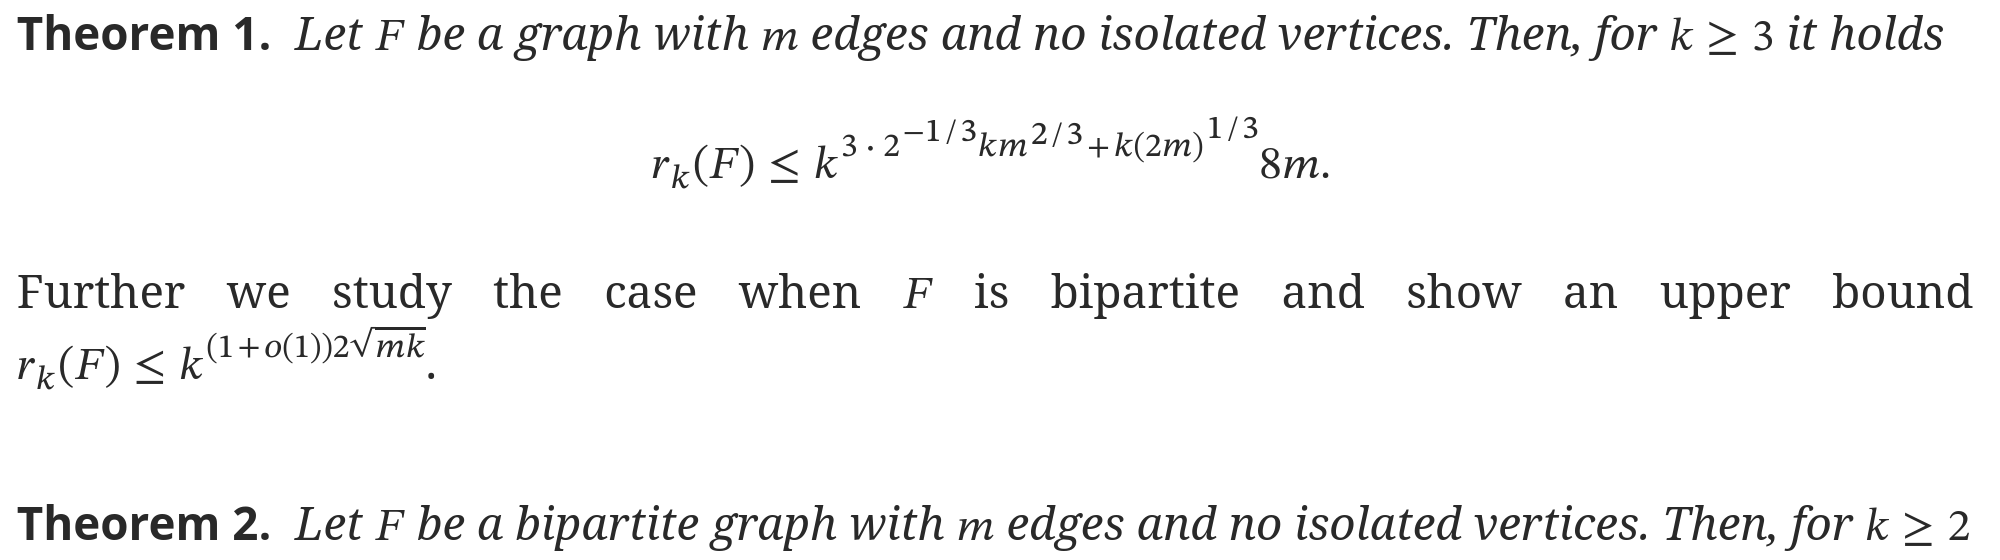
\includegraphics[scale=0.25]{theorems_1311_5471.png}};
        \node at (5, -4) {\examplecite{johst2013multicolor}};
        % \node[draw] (doc) at (0, -3) {\bf Fixed/frozen corpus};
        \draw[->,dashed] (db) -- (doc);
        \pause
        \node[draw,fill=yellow!70,opacity=0.9] at (0, -3) {\bf Fixed/frozen corpus};
    \end{tikzpicture}

%     \begin{itemize}
%         \item \textbf{Spotter:} specialized tool for finding a particular type of annotation
%         \item Examples: Identifier declarations, quantity expressions,
%             paragraph type (theorem/definition/\textellipsis), \textellipsis
%         \item Simple spotters, hybrid spotters, meta spotters
%     \end{itemize}
    % pictures with annotations (simple spotter, hybrid spotter, meta spotter)
    % e.g. "concept references and quantities", "variable declarations", "conflict resolution var. occurrence vs unit"
\end{frame}


\begin{frame}
    \frametitle{What is the problem?}
    \begin{enumerate}
        \item Getting a corpus:\com{Working with PDF is difficult}
            \begin{itemize}
                \item arXMLiv/ar5iv dataset~\cite{SML:arXMLiv:2020}\com{convert \texttt{.tex} to \texttt{.html}}
                \item SIGMathLing~\cite{SIGMathLing:on}\com{NDA-cooperative to work around licensing issues}
            \end{itemize}
        \item Re-inventing the wheel:
            \begin{itemize}
                \item Need to obtain plaintext representation
                \item Need to store annotations
                \item Need to create manual annotations\com{for training/evaluation}
            \end{itemize}
        \item Cannot re-use existing annotations/combine results:
            \begin{itemize}
                \item No agreed-upon annotation format
                \item Original documents modified
            \end{itemize}
    \end{enumerate}
\end{frame}


\begin{frame}
    \frametitle{A new annotation standard}
    \begin{itemize}
        \item Supports development of re-usable tools, datasets and benchmarks
        \item Uses RDF (Resource Description Framework)\com{$\exists$ databases, query language (SPARQL), serialization formats}
        \item Based on W3C Web Annotation Recommendations
    \end{itemize}
    % based on RDF, Web Annotation Standard, ...
    \pause
    \vspace{1.5em}
    \rule{\textwidth}{0.4pt}\\
    \vspace{1.5em}
    \textbf{RDF Primer}\\[1em]
    \begin{tabular}{ll}
        subject-predicate-object triple\quad\quad\quad &
        \texttt{ex:anno1 rdf:type oa:Annotation} \\[1em]
        directed graph &
        \begin{tikzpicture}[baseline={([yshift=-.5ex]current bounding box.center)}]
            \node[urinode] (s) at (0, 0) {{ex:anno1}};
            \node[urinode] (o) at (4.5, 0) {{oa:Annotation}};
            \draw[normaledge] (s) --node[above]{{rdf:type}} (o);
        \end{tikzpicture}\\
    \end{tabular}
\end{frame}


\begin{frame}
    \frametitle{Annotation structure (following W3C Web Annotation Recommendation)}
    \centering
    % body, target, meta-data
    \begin{tikzpicture}[yscale=1.8]
        \node[urinode,annotation] (anno) at (0, 0) {ex:anno1};
        
        \node[typenode] (annot) at (-4.5, 1) {oa:Annotation};
        \draw[typeedge] (anno) --node[fill=white]{rdf:type} (annot);
        \node[urinode] (author) at (0, 1) {\textellipsis};
        \draw[normaledge] (anno) --node[fill=white,pos=0.4]{dcterms:creator} (author);
        \node[urinode] (created) at (4.5, 1) {\textellipsis};
        \draw[normaledge] (anno) --node[fill=white,pos=0.6]{dcterms:created} (created);

        \onslide<2-3>{
            \node (targ) at (-3, -1) {\textellipsis};
            \draw[normaledge] (anno) --node[fill=white]{oa:hasTarget} (targ);
            % \node[urinode] (targ) at (-3, -1) {ex:target1};
            % \draw[normaledge] (anno) --node[fill=white]{oa:hasTarget} (targ);
            % \node (targ1) at (-4,-1.5) {\textellipsis};
            % \node (targ2) at (-2,-1.5) {\textellipsis};
            % \draw[normaledge] (targ) -- (targ1);
            % \draw[normaledge] (targ) -- (targ2);

            % \node[urinode] (body) at (3,-1) {ex:body1};
            \node (body) at (3,-1) {\textellipsis};
            \draw[normaledge] (anno) --node[fill=white]{oa:hasBody} (body);
        }
    \end{tikzpicture}
    \onslide<3>{
        \vspace{2em}\par
        \begin{columns}
            \begin{column}{0.5\textwidth}
                \centering
                
\includegraphics[width=\textwidth]{bipart_graph.png}
                \\\hfill\examplecite{johst2013multicolor}
            \end{column}
            \begin{column}{0.5\textwidth}
                \centering
                \texttt{wd:Q174733}\\
                (WikiData: bipartite graph)
            \end{column}
        \end{columns}
    }
\end{frame}

\begin{frame}
    \frametitle{Example annotation bodies: simple body}
    \centering
    \hfill\examplecite{johst2013multicolor}
    
\includegraphics[width=0.8\textwidth]{bipart_graph.png}
    \par
    \begin{tikzpicture}
        \node[urinode,annotation] (anno) at (0, 2) {ex:anno1};
        \node[urinode,body] (bipart_graph) at (0, 0) {wd:Q174733};
        \node (target) at (0, 4) {};
        \draw[normaledge] (anno) --node[fill=white]{oa:hasBody} (bipart_graph);
        \draw[normaledge] (anno) --node[fill=white]{oa:hasTarget} (target);
        \pause
        \node[urinode,black!70] (multipartgraph) at (-4, 1.5) {wd:Q1718082};
        \draw[normaledge,black!70] (bipart_graph) --node[fill=white]{subclass of} (multipartgraph);
        \node[literal,black!70] (labelfr) at (4, 1.5) {``graphe biparti''\makeatletter @\makeatother fr};
        \node[literal,black!70] (labelde) at (4, -1.5) {``bipartiter Graph''\makeatletter @\makeatother de};
        \draw[normaledge,black!70] (bipart_graph) --node[fill=white]{rdfs:label} (labelfr);
        \draw[normaledge,black!70] (bipart_graph) --node[fill=white]{rdfs:label} (labelde);
        \node[urinode,black!70] (graphtheo) at (-3.5, -1.5) {wd:Q131476};
        \draw[normaledge,black!70] (bipart_graph) --node[fill=white]{studied by} (graphtheo);
        \node[black!70] (dots1) at (-5.5, 0.6) {\textellipsis};
        \draw[normaledge,black!70] (multipartgraph) -- (dots1);
        \node[black!70] (dots2) at (-5.1, -0.5) {\textellipsis};
        \draw[normaledge,black!70] (graphtheo) -- (dots2);
        \node[black!70] (dots3) at (-0.5, -1.7) {\textellipsis};
        \draw[normaledge,black!70] (graphtheo) -- (dots3);
    \end{tikzpicture}
\end{frame}

\begin{frame}
    \frametitle{Example annotation bodies: complex body}
    \centering
    \hfill\examplecite{Althaus_2022}\\
    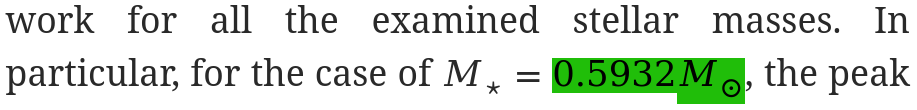
\includegraphics[width=0.65\textwidth]{solarmass_2205_14126.png}
    \vspace{-0.5em}\par
    \begin{tikzpicture}
        \node[urinode,annotation] (anno) at (0, 2) {ex:anno2};
        \node[bnode,body] (body) at (0, 0) {};
        \node (target) at (3, 4) {};
        \draw[normaledge] (anno) --node[fill=white]{oa:hasBody} (bipart_graph);
        \draw[normaledge] (anno) --node[fill=white]{oa:hasTarget} (target);
        \node[typenode,body] (measure) at (-4, 1.7) {om:Measure};
        \node[literal,body] (scalar) at (-3, -1.7) {0.5932};
        \node[urinode,body] (unit) at (3.5, -1.7) {om:solarMass};
        \draw[normaledge] (body) --node[fill=white]{rdf:type} (measure);
        \draw[normaledge] (body) --node[fill=white]{om:hasNumericalValue} (scalar);
        \draw[normaledge] (body) --node[fill=white]{om:hasUnit} (unit);
        \node[urinode,black!70] (dim) at (5, 0) {om:mass-Dimension};
        \draw[normaledge,black!70] (unit) --node[fill=white]{om:hasDimension} (dim);
    \end{tikzpicture}
\end{frame}

\begin{frame}
    \frametitle{Example annotation bodies: linked bodies}
    \begin{tikzpicture}
        \node (frag) at (0, 0) {\begin{tabular}l\examplecite{johst2013multicolor}\\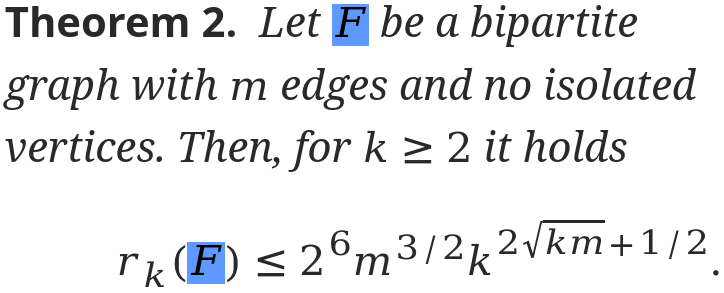
\includegraphics[scale=0.3]{declwithocc.png}\end{tabular}};
        \pause
        \node[urinode,annotation] (anno3) at (2, 3.2) {ex:anno3};
        \node (target3) at (0, 1.2) {};
        \draw[normaledge] (anno3) --node[fill=white]{oa:hasTarget} (target3);
        \node[bnode,body] (body3) at (5, 1.7) {};
        \draw[normaledge] (anno3) --node[fill=white]{oa:hasBody} (body3);
        \node[typenode,body] (type3) at (7, 3.2) {do:IdDecl};
        \draw[normaledge] (body3) --node[fill=white]{rdf:type} (type3);
        \node[urinode,body] (quant) at (8, 0.3) {do:Univ};
        \draw[normaledge] (body3) --node[fill=white]{do:quant} (quant);

        \pause
        \node[urinode,fill=yellow] (id) at (5, 0) {ex:id1};
        \draw[normaledge] (body3) --node[fill=white]{do:id} (id);

        \pause
        \node[urinode,annotation] (anno4) at (2, -3.2) {ex:anno4};
        \node (target4) at (-1.2, -1.2) {};
        \draw[normaledge] (anno4) --node[fill=white]{oa:hasTarget} (target4);
        \node[bnode,body] (body4) at (5, -1.7) {};
        \draw[normaledge] (anno4) --node[fill=white]{oa:hasBody} (body4);
        \node[typenode,body] (type4) at (7, -3.2) {do:IdOcc};
        \draw[normaledge] (body4) --node[fill=white]{rdf:type} (type4);
        \draw[normaledge] (body4) --node[fill=white]{do:id} (id);
    \end{tikzpicture}
\end{frame}


\begin{frame}[fragile]
    \frametitle{Annotation Targets}
    % \lstinline[literate={≤}{$\le$}1]|<p>it follows that <math><mrow><msqrt><mi>x</mi></msqrt><mo>≤</mo><mn>1</mn></mrow></math>.</p>|
%     \lstinline[literate={≤}{$\le$}1]|<p>It follows that <math><mrow><msqrt><mi>x</mi></msqrt><mo>≤</mo>...|
%     \textit{``It follows that $\sqrt x \le 1$.''}
%     \vspace{1em}\par

    \centering
    \footnotesize
    \begin{tikzpicture}[xscale=-1]
        % anno nodes
        \node[urinode,annotation] (anno) at (0, 0) {ex:anno0};
        % \node[typenode] (annotype) at (1, 1.5) {oa:Annotation};
        % \node (creator) at (-3, 1.5) {...};
        % % anno edges
        % \draw[typeedge] (anno) --node[fill=white]{rdf:type} (annotype);
        % \draw[normaledge] (anno) --node[fill=white]{dcterms:creator} (creator);


        % body nodes
        \node[bnode,body] (body) at (-2, -1.3) {\textellipsis};
        % \node[typenode] (bodytype) at (-1.5, -3) {om:Measure};
        % \node[bnode] (unit) at (-4, -4) {om:gramPerCubicmetre};
        % \node[literal] (scalar) at (-4, 0.75) {1292.1};

        % body edges
        \draw[normaledge] (anno) --node[fill=white]{oa:hasBody} (body);
        % \draw[typeedge] (body) --node[fill=white]{rdf:type} (bodytype);
        % \draw[normaledge] (body) --node[fill=white]{om:hasNumericalValue} (scalar);
        % \draw[normaledge] (body) --node[fill=white]{om:hasUnit} (unit);
        % om:hasNumericalValue
        % om:hasUnit

        % target nodes
        \node[urinode,target] (target) at (4, -1.5) {ex:target0};
        \node[urinode,target] (src) at (5, 0) {ex:document.html};
        \draw[normaledge] (anno) --node[fill=white]{oa:hasTarget} (target);
        \draw[normaledge] (target) --node[fill=white]{oa:hasSource} (src);

        \onslide<2-4>{
            \node[typenode,target] (pathseltype) at (7.2, -2.3) {sb:PathSelector};
            \node[bnode,target] (pathsel) at (5.2, -3.75) {};
            \node[literal,target] (pathselstart) at (2.5, -5.5) {``after-node(/html/.../math[3])''};
            \node[literal,target] (pathselend) at (7.5, -5.5) {``char(/html/.../p[2], 819)''};

            \draw[normaledge] (target) --node[fill=white]{oa:hasSelector} (pathsel);
            \draw[normaledge] (pathsel) --node[fill=white]{sb:startPath} (pathselend);
            \draw[normaledge] (pathsel) --node[fill=white]{sb:endPath} (pathselstart);
            \draw[typeedge] (pathsel) --node[fill=white]{rdf:type} (pathseltype);
        }

        \onslide<3>{
            \node[draw,fill=yellow!70, fill opacity=0.9, inner sep=0.5cm] at (2.0, -3) {
                    \large
                    \begin{tabular}l
                        \lstinline[literate={≤}{$\times$}1]|<p>The integer solutions of|\\
                        \lstinline[literate={≤}{$\times$}1]|<math><mrow><msqrt><mi>x</mi></msqrt><mo>≤</mo>...|
                    \end{tabular}
            };
        }

        \onslide<4>{
            \node[typenode,target] (offseltype) at (0.5, -1.5) {sb:OffsetSelector};
            \node[bnode,target] (offsel) at (1, -3) {};
            \node[literal,target] (offselstart) at (2.3, -4.5) {1592};
            \node[literal,target] (offselend) at (0, -4.5) {1605};
            \draw[normaledge] (offsel) --node[fill=white]{oa:start} (offselstart);
            \draw[normaledge] (offsel) --node[fill=white]{oa:end} (offselend);
            \draw[normaledge] (target) --node[fill=white]{oa:hasSelector} (offsel);
            \draw[typeedge] (offsel) --node[fill=white]{rdf:type} (offseltype);
        }
    \end{tikzpicture}
\end{frame}



\begin{frame}
    \frametitle{Prototype datasets and imported datasets}
    \begin{itemize}
        \item Imported datasets:
            \begin{itemize}
                \item Quantity expressions dataset~\cite{Rabenstein:msc17}
                \item Formula grounding dataset~\cite{asakura-miyao-aizawa:2022:LREC}
                \item Paragraph classification dataset~\cite{ginev-miller-2020-scientific}
            \end{itemize}
        \item Generated datasets (prototype spotters)\com{https://github.com/jfschaefer/spotters}
            \begin{itemize}
                \item Part-of-speech tags
                \item References to math concepts
                \item Variable declarations
            \end{itemize}
        \item Stats from running last two spotters:
            \begin{itemize}
                \item 100\,000 documents
                \item 50 million annotations
                \item 800 million triples
                \item loading into triple store: several hours
            \end{itemize}
    \end{itemize}
\end{frame}


\begin{frame}[fragile]
    \frametitle{Querying}
    {\centering\itshape
        \colorbox{yellow}{
    ``Papers about group theory that have theorems mentioning rational numbers''
}
    \par}
    \footnotesize
\begin{lstlisting}[language=SPARQL]
# prefix declarations ommitted for conciseness
SELECT DISTINCT ?paper WHERE {
  # make sure that ?paper is about group theory
  ?paper sb:isBasedOn/^oa:hasTarget/oa:hasBody/rdf:value arxivcat:math\.GR .
  # find theorems in ?paper and look up their offsets
  ?theorem_anno oa:hasBody/rdf:value sbp:Theorem .
  ?theorem_anno oa:hasTarget [
    oa:hasSource ?paper ;
    oa:hasSelector [ a sb:OffsetSelector ; oa:start ?t_start ; oa:end ?t_end ; ]
  ] .
  # Same with mentions of rational numbers (offsets ?q_start, ?q_end)
  ?q_anno oa:hasBody/rdf:value <http://www.wikidata.org/entity/Q1244890> .
  ?q_anno oa:hasTarget [
    oa:hasSource ?paper  ;
    oa:hasSelector [ a sb:OffsetSelector ; oa:start ?q_start ; oa:end ?q_end ; ]
  ] .
  # make sure that mention is inside theorem
  FILTER (?t_start < ?q_start && ?t_end > ?q_end)
}
\end{lstlisting}

\end{frame}



\begin{frame}
    \frametitle{Selling points}
    \begin{itemize}
        \item Conversion to/from JSON\com{no need to learn RDF/SPARQL}
        \item Ecosystem of tools:
            \begin{itemize}
                \item Tool for manual annotation\com{MathUI workshop at 2:00 pm today}
                \item Pre-processing for NLP
                \item More to come?
            \end{itemize}
        \item Datasets
            \begin{itemize}
                \item for evaluation
                \item for comparison
                \item for training
                \item to build upon
            \end{itemize}
        \item Public SPARQL endpoint
    \end{itemize}
    % Concern   ->   answer
    % No datasets exist - what do I get concretely?    ->   annotation tool
    % I don't know RDF/can't use it in my environment   ->   JSON-LD
    % But I need dataset XYZ in a different format   ->   conversion?
    \begin{tikzpicture}[remember picture,overlay]
        \node[xshift=-4.5cm,yshift=2cm] at (current page.south east) {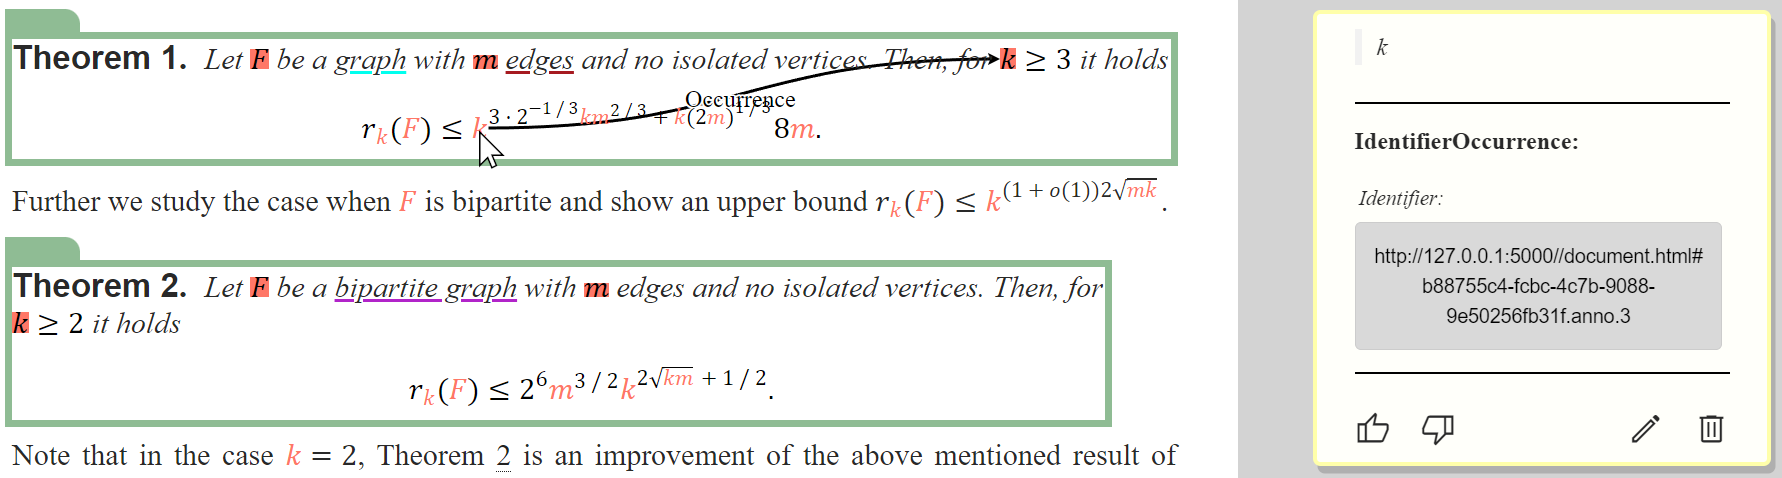
\includegraphics[scale=0.35]{workflow_3.png}};
    \end{tikzpicture}
\end{frame}


\begin{frame}
    \frametitle{Conclusion}
    An annotation standard for STEM documents
    \begin{itemize}
        \item based on semantic web technologies\com{RDF, SPARQL, Web Annotation Standard}
        \item compatible with a wide range of annotation tasks
        \item to create diverse, re-usable annotation datasets and benchmarks
        \item to develop an ecosystem of tools around that standard
        \item to ultimately enable the development of semantic services\com{active documents, formula search, \textellipsis}
    \end{itemize}
\end{frame}

\appendix   % stop page number count

\begin{frame}[allowframebreaks,t]
    \frametitle{References}
    \printbibliography
\end{frame}

\end{document}
